\chapter{Methodology}

\section{Study sites and experimental setting}
\label{sec:StudysitesAndExperimentalSetting}

In order to assess the climatic effect on soil and its interactions with biocrusts, five study sites distributed between latitudes from \ang{26;6}~S to \ang{37;48}~S and over \SI{1315}{\kilo\meter} were established in the Chilean Coastal Range (Figure \ref{fig:location-map}): Pan de Azúcar National Park (PdA), Santa Gracia Natural Reserve (SG), Quebrada de Talca Private Reserve (QdT), La Campana National Park (LC) and Nahuelbuta National Park (NA), corresponding to arid, coastal semi-arid, inland semi-arid, Mediterranean and humid climates, respectively \citep{Bernhard2018}.

\begin{figure}[H]
	\centering
	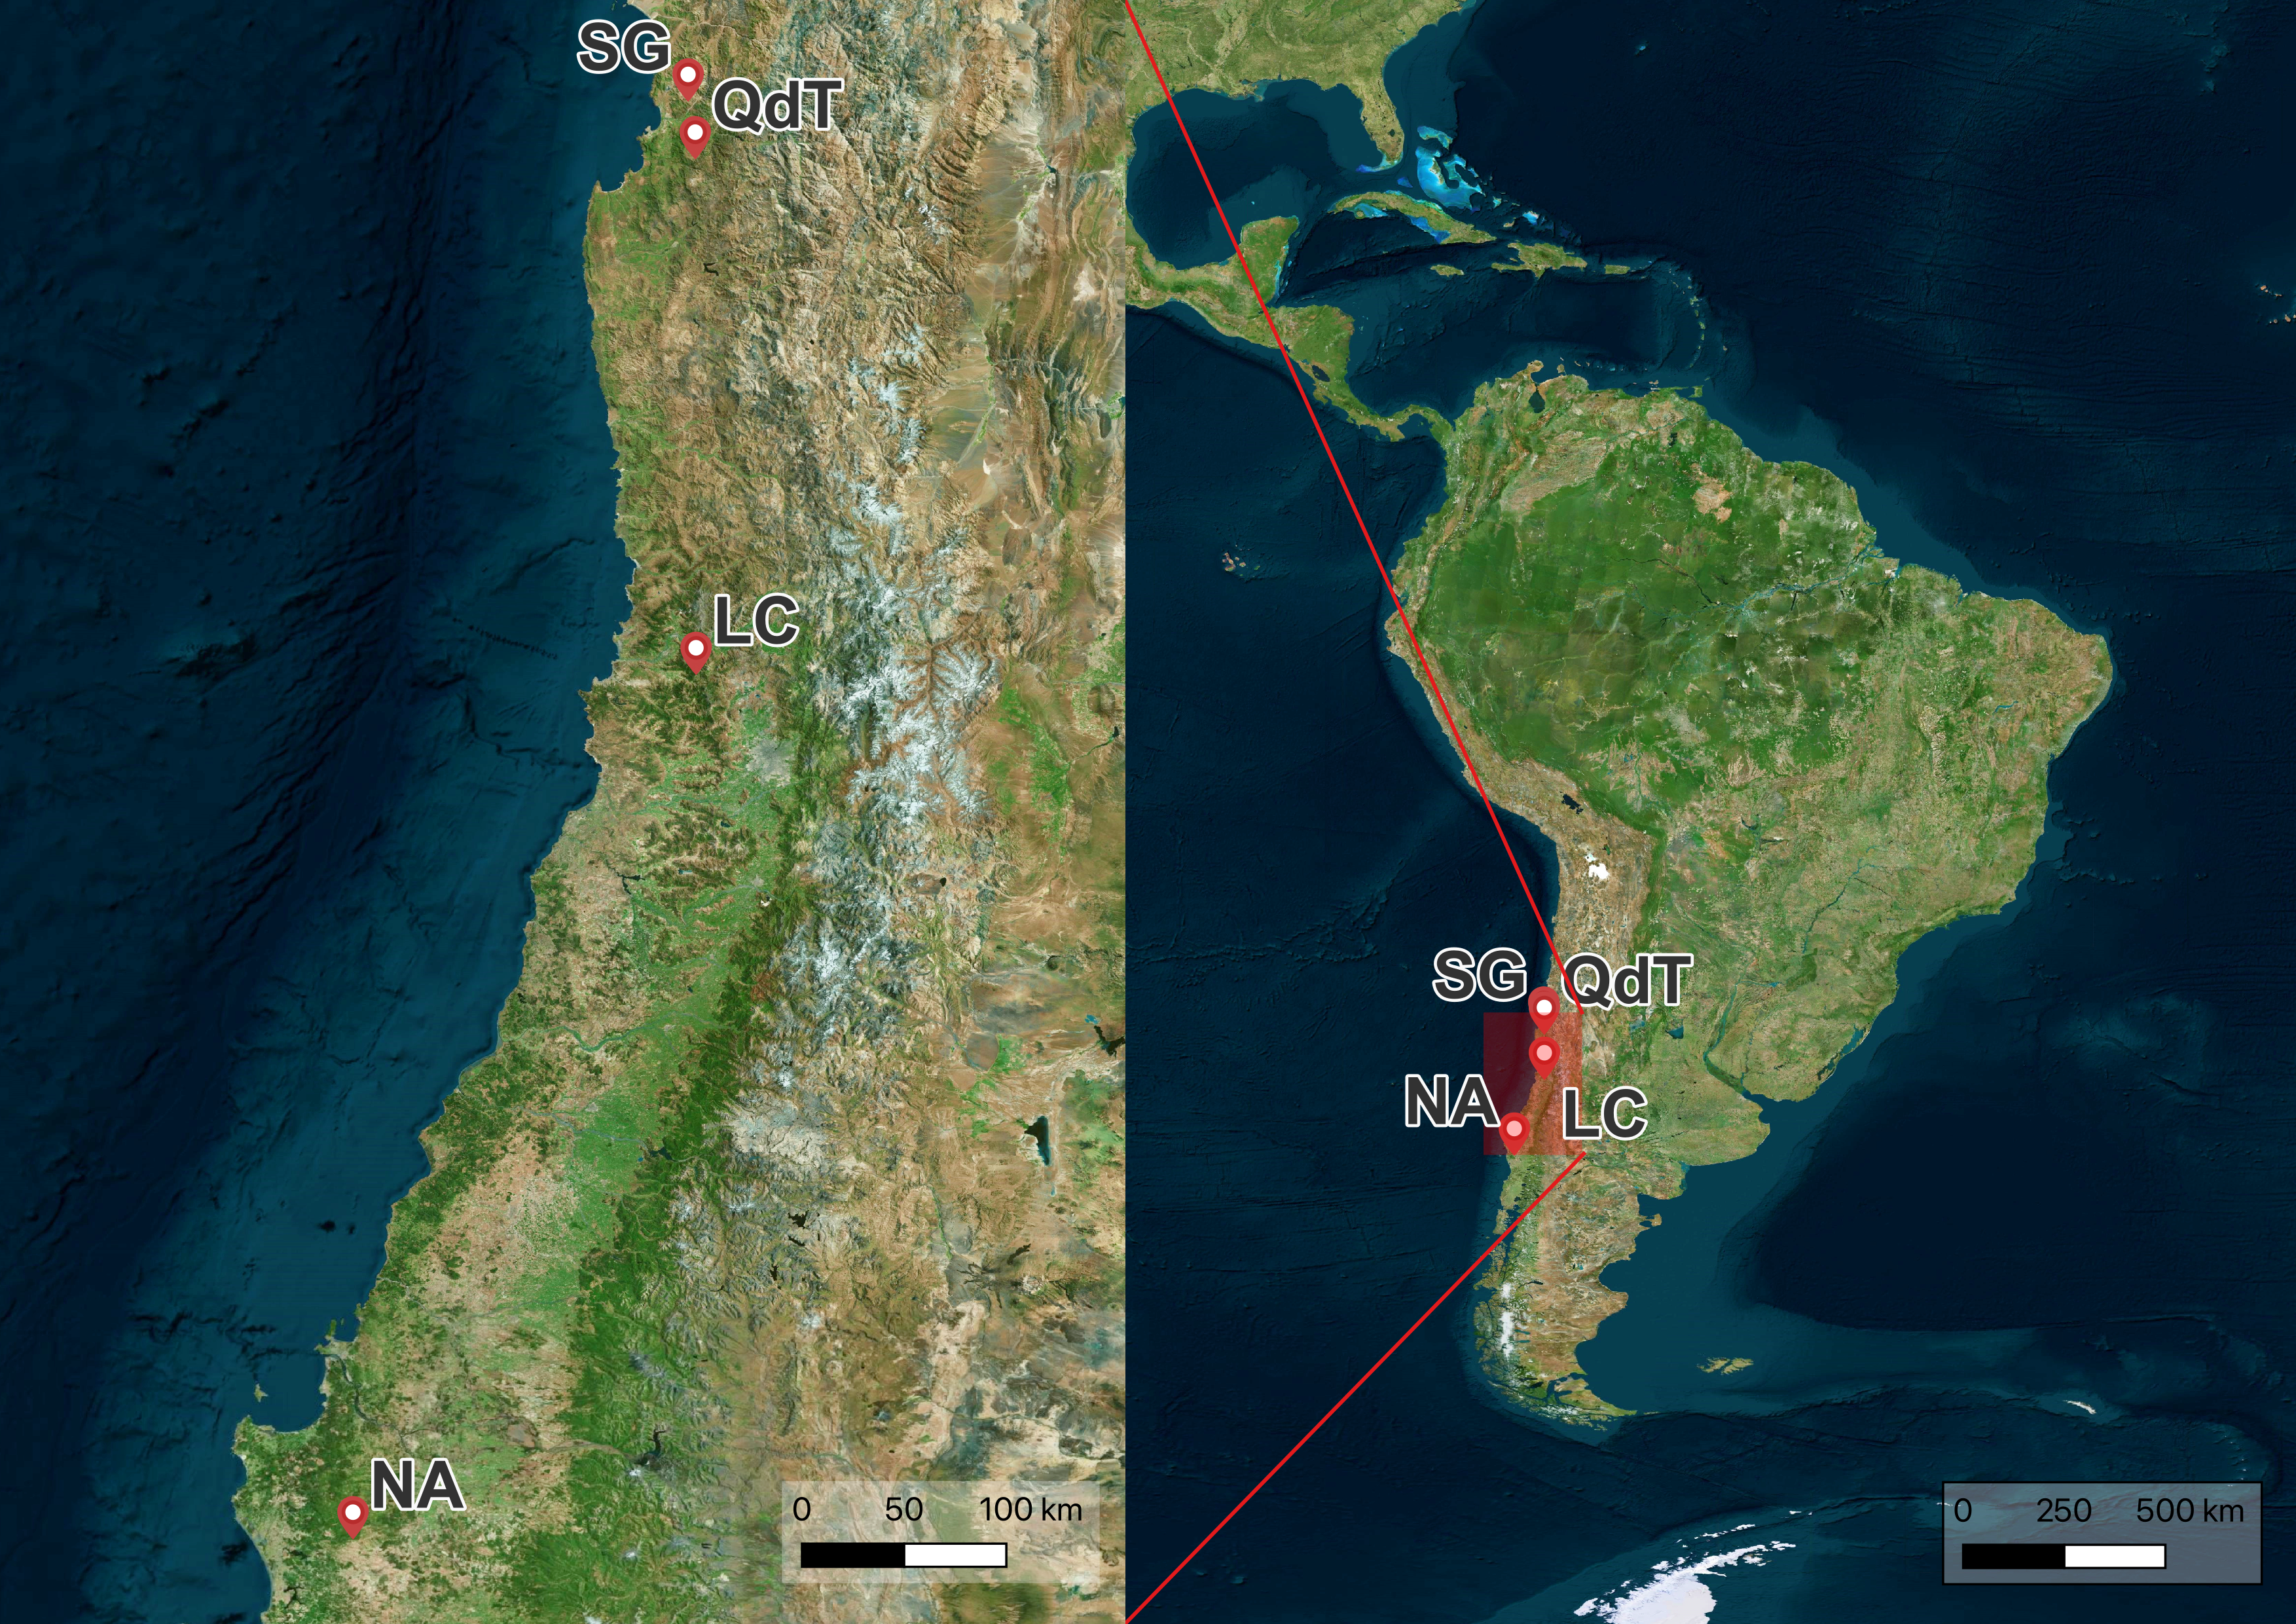
\includegraphics[width=1\textwidth]{img/location-map.png}
	\caption[Location of study sites relative to South America]{Location of study sites relative to South America. From north to south: Pan de Azúcar (PdA), Santa Gracia (SG), Quebrada de Talca (QdT), La Campana (LC), and Nahuelbuta (NA).}
	\label{fig:location-map}
\end{figure}

The study sites are comparable in geology, geomorphology, land use, and influence of glaciers and volcanoes \citep{Bernhard2018}. The parent material in all the study sites is granitoid \citep{Bernhard2018}. The dominant topography is generally fluvial valleys, and the sites had no glacial influence during the last glaciation \citep{Hulton2002}. The sites are located within nature protection areas, with limited anthropogenic influence compared to the surrounding areas. Despite this, cattle occasionally enter these locations, and goats, mules, and donkeys have been reported to SG \citep{Armesto2007}.

The mean annual temperature (MAT) decreases from north to south (PdA: \SI{16.8}{\celsius}, SG: \SI{13.7}{\celsius}, QdT: \SI{14.3}{\celsius}, LC: \SI{14.1}{\celsius}, NA: \SI{6.6}{\celsius}). The mean annual precipitation (MAP) in the study sites increases from north to south (PdA: \SI{12}{\milli\metre\,\year^{-1}}, SG: \SI{66}{\milli\metre\,\year^{-1}}, QdT: \SI{109}{\milli\metre\,\year^{-1}}, LC: \SI{367}{\milli\metre\,\year^{-1}}, NA: \SI{1469}{\milli\metre\,\year^{-1}}) with similar rainfall distribution mostly concentrated in winter months (May to August) \citep{Bernhard2018,Santibnez2017}. The elevation of the sites increases from north to south (PdA: \SIrange{329}{351}{\meter}, SG: \SIrange{642}{720}{\meter}, QdT: \SIrange{565}{611}{\meter}, LC: \SIrange{708}{732}{\meter}, NA: \SIrange{1200}{1270}{\meter}). Paleoclimate modeling studies \citep{Mutz2018} indicate that these climate patterns have been persistent since the late Pliocene; thus, the study sites represent the long-term impact of climate on the soil \citep{Ewing2006}. \citet{Bernhard2018} classified soils in the study sites as Regosols in PdA, Cambisols for SG and LC, and Umbrisols in NA. In general, pedogenic properties such as soil depth, clay content, organic matter accumulation, porosity, and activity ratio are positively correlated with site humidity \citep{Bernhard2018}.

For each of the 5 study sites (Figure \ref{fig:location-panel}), 5 plots of \SI{1}{\meter}~$\times$~\SI{1}{\meter} were set up as replicates (P1 to P5). Each plot was assigned in the top-slope position with a south-facing exposition, considering a high presence of site-typical biocrust communities, similar slope and aspect, lack of anthropogenic disturbance, and a maximum distance of \SI{30}{\meter} between each plot. Within each plot, patches with the highest available biocrust cover were included as treatment BSC+, and nearby bare soil without biocrust cover was defined as control (BSC-). \newline

\begin{figure}[ht!]
	\centering
	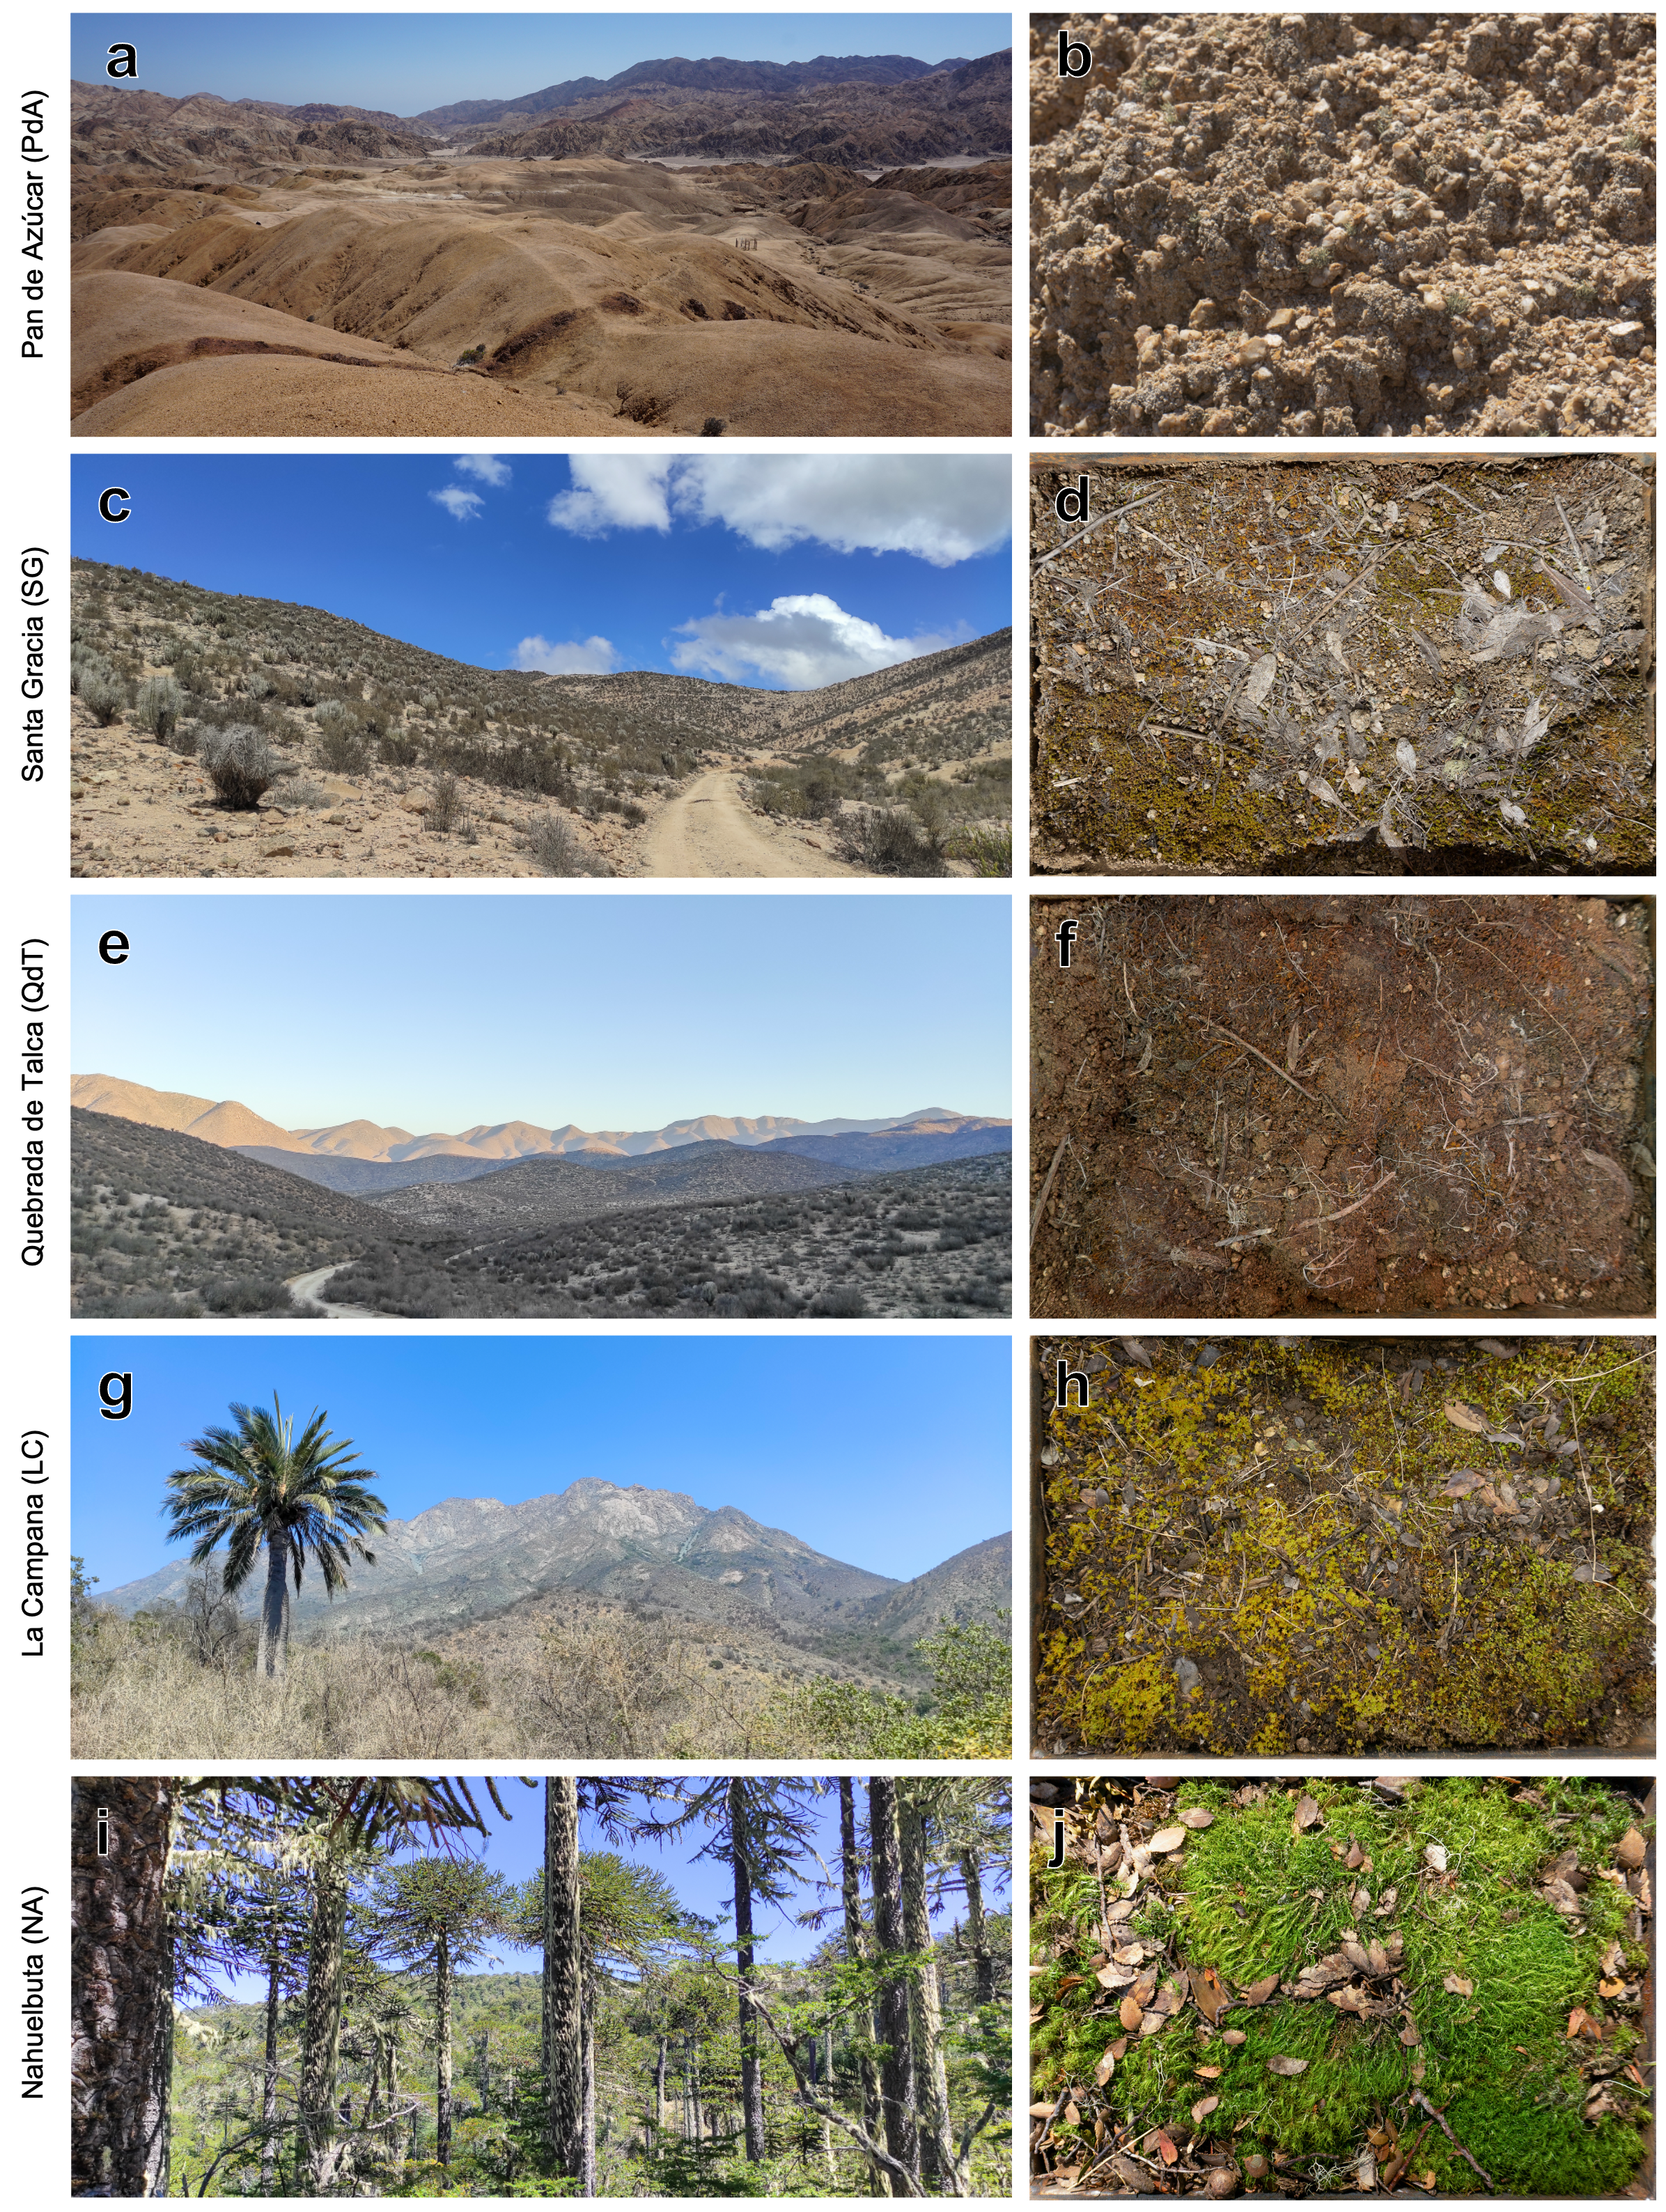
\includegraphics[width=1\textwidth]{img/location-panel.png}
	\caption[General view and biocrust sampled for the study sites]{General view (a, c, d, g, and i) and sampled biocrust (b, d, f, h, and j) of PdA, SG, QdT, LC, and NA.}
	\label{fig:location-panel}
\end{figure}

\FloatBarrier

\section{Field methods}
\label{sec:FieldMethods}
\subsection{Biocrust sampling and characterization}

In a first field campaign during March 2019, biocrust patches of approximately \SI{100}{\centi\metre^{2}} were collected in PdA, SG, LC and NA and identified according to \citet{Lange2016}. The patches were collected in the field by carefully detaching the biocrust layer, removing the loose soil, and storing it in paper envelopes after air-drying for every research plot. \citet{Samolov2020} describes a biocrusts dominance in PdA with cover of up to 40\%. The other study sites are dominated by higher vegetation that limits the cover of biocrust up to 15\% in SG and 5\% in LC and NA. Sampled communities showed all typical biocrust classes from cyanobacteria, algae, fungi, lichens, liverworts, and mosses. The species composition further showed a graduating change from lichen-dominating biocrusts in the northernmost site to bryophyte-dominating biocrusts in the southernmost site. Biocrusts in NA were specifically found in zones of forest soil disturbance. Bryophyte-dominated biocrusts were sampled with rhizoids down to \SI{5}{\milli\metre} depth; all other communities were down to \SI{2}{\milli\metre}. Dominant macroscopic biocrust species were determined for each of the four sites to the genus level by morphological characteristics using a stereomicroscope (Leitz TS, Wetzlar, Germany), a transmitted-light microscope (Leitz Laborlux S, Wetzlar, Germany), and ultraviolet light. Species groups were separated into bryophytes \citep{Ardiles2014,BednarekOchyra2001,Cuvertino2012,He1998,Lightowlers2013} and lichens \citep{Galloway2007} and assigned to the different regions (Table \ref{tab:taxonomical_composition}). \citet{Bernhard2018}, based on morphological identification of enrichment cultures, reported that the biocrusts of the four studied sites were composed of 18 to 15 species of algae and cyanobacteria; where the richness of green algae increased, while the richness of cyanobacteria decreased with increasing humidity and decreasing mean annual temperature. While \citet{Samolov2020}, based on morphological and molecular traits, reported 18 species in PdA, 26 species in SG, 40 species in LC, and 27 species in NA.

\begin{table}[ht!]
\centering
\caption{Taxonomical composition of mosses and lichens in the biological soil crust for the study sites along the climatic gradient.}
\resizebox{\textwidth}{!}{%
\begin{tabular}{lllc}
\hline
\textbf{Site / Division} & \textbf{Family} & \textbf{Genus} & \textbf{No. species} \\
\hline
\textbf{PdA} & & & \\
Lichens & Cladoniaceae & \textit{Cladonia} sp. & 2 \\
        & Verrucariaceae & \textit{Placidium} sp. & 2 \\
        & Lecanoraceae & \textit{Lecidella} sp. & 1 \\
        & Rhizocarpaceae & \textit{Rhizocarpon} sp. & 1 \\
\hline
\textbf{SG} & & & \\
Mosses & Pottiaceae & \textit{Syntrichia} sp. & 2 \\
       & Pottiaceae & \textit{Tortella} sp. & 2 \\
Unidentified lichens & & & 2 \\
\hline
\textbf{LC} & & & \\
Mosses & Bartramiaceae & \textit{Philonotis} sp. & 1 \\
       & Bryaceae & \textit{Bryum} sp. & 1 \\
       & Pottiaceae & \textit{Syntrichia} sp. & 2 \\
       & Pottiaceae & \textit{Tortella} sp. & 2 \\
Unidentified mosses and lichens & & & 2 + 1 \\
\hline
\textbf{NA} & & & \\
Mosses & Amblystegiaceae & \textit{Acrocladium} sp. & 1 \\
       & Amblystegiaceae & \textit{Amblystegium} sp. & 1 \\
       & Bartramiaceae & \textit{Bartramia} sp. & 1 \\
       & Bryaceae & \textit{Bryum} sp. & 1 \\
       & Dicranaceae & \textit{Campylopus} sp. & 2 \\
       & Pterigynandraceae & \textit{Myurella} sp. & 1 \\
Unidentified liverworts, lichens, fungi & & & 2 + 2 + 1 \\
\hline
\end{tabular}}
\label{tab:taxonomical_composition}
\end{table}

\FloatBarrier

\subsection{Soil sampling}

Soil sampling campaigns were primarily conducted during the austral dry season (typically January-April) to capture baseline soil conditions prior to the onset of winter precipitation. Specific sampling approaches were adapted based on the objectives of individual studies. For investigations concerning aggregate stability, moisture regime effects, and general baseline characterization across the full gradient (PdA, SG, LC, NA), bulk topsoil samples (\SIrange{0}{5}{\centi\metre} depth) were collected from each plot on mid-slope, south-facing locations using metal-core augers or by sampling from shallow soil pits (Manuscripts 1 and 4). These samples were processed in the field by sieving ($<$\SI{2}{\milli\metre}), another batch of samples was sieved and sterilized with ethanol, before being homogenized per site or kept discrete per plot depending on the experimental design and subsequently stored at \SI{4}{\celsius} pending laboratory analysis. For studies focusing on initial soil formation and rhizosphere/detritusphere dynamics (PdA, SG), distinct soil horizons (A horizon: \SIrange{0}{2}{\centi\meter}/\SIrange{0}{3}{\centi\meter}; B horizon: \SIrange{2}{3}{\centi\meter}/\SIrange{25}{40}{\centi\meter}) where sampled from excavated soil pits (Manuscripts 3 and 5). Processing involved similar steps: sieving ($<$\SI{2}{\milli\metre}), homogenization per horizon and site, and storage at \SI{4}{\celsius}.

\subsection{Rainfall simulations}

Following observations of limited soil stabilization at PdA, further rainfall simulation experiments were conducted during subsequent expeditions in 2020 and 2022 at SG, Quebrada de Talca (QdT), LC, and NA. Five \SI{1}{\meter}~$\times$~\SI{1}{\meter} plots were established as replicates at each of the four sites, consistently located on south-facing top slopes. Plot selection considered the presence of representative biocrust communities, similar slope and aspect, minimal anthropogenic disturbance, and a maximum inter-plot distance of \SI{30}{\meter}. Within each plot, runoff plots (ROPs) were established in areas with maximum biocrust cover for biocrust-present (BSC+) treatments, and adjacent biocrust-free (BSC-) locations served as controls. The experimental design was a factorial completely randomized design, incorporating four sites (SG, QdT, LC, and NA) (Figure \ref{fig:location-panel}), two biocrust conditions (BSC+ and BSC-), five replicate plots (P1-P5), and three technical replicate ROPs (R1-R3) per plot. This resulted in a total of eight treatments (site × biocrust) with 15 samples per treatment (plot $\times$ technical replicate), yielding a total sample size of n = 60.

Undisturbed soil samples for rainfall simulation were collected (Figures \ref{fig:sampling-panel}b and \ref{fig:sampling-panel}c), using piercing frames (\SI{20}{\meter}~$\times$~\SI{30}{\meter}~$\times$~\SI{7}{\meter}) (Figure \ref{fig:sampling-panel}a) and carefully installed into infiltration boxes to minimize surface and subsurface disturbance (Figure \ref{fig:sampling-panel}d). These steel boxes, designed with a triangular surface runoff gutter and a bottom outlet, captured both runoff and percolated water. Soil water content was measured using a TDR probe (Delta-T Devices Ltd. Cambridge, UK), averaging three measurements adjacent to each ROP. Biocrust cover in BSC+ ROPs was assessed using perpendicular photographs taken with a digital camera (Sony ILCE-6000, SELP1650 lens; Tokyo, Japan). Photographs were analyzed using the grid-quadrat method with a 100-subdivision grid, and biocrusts were identified visually \citep{Belnap2001}.

\begin{figure}[ht!]
	\centering
	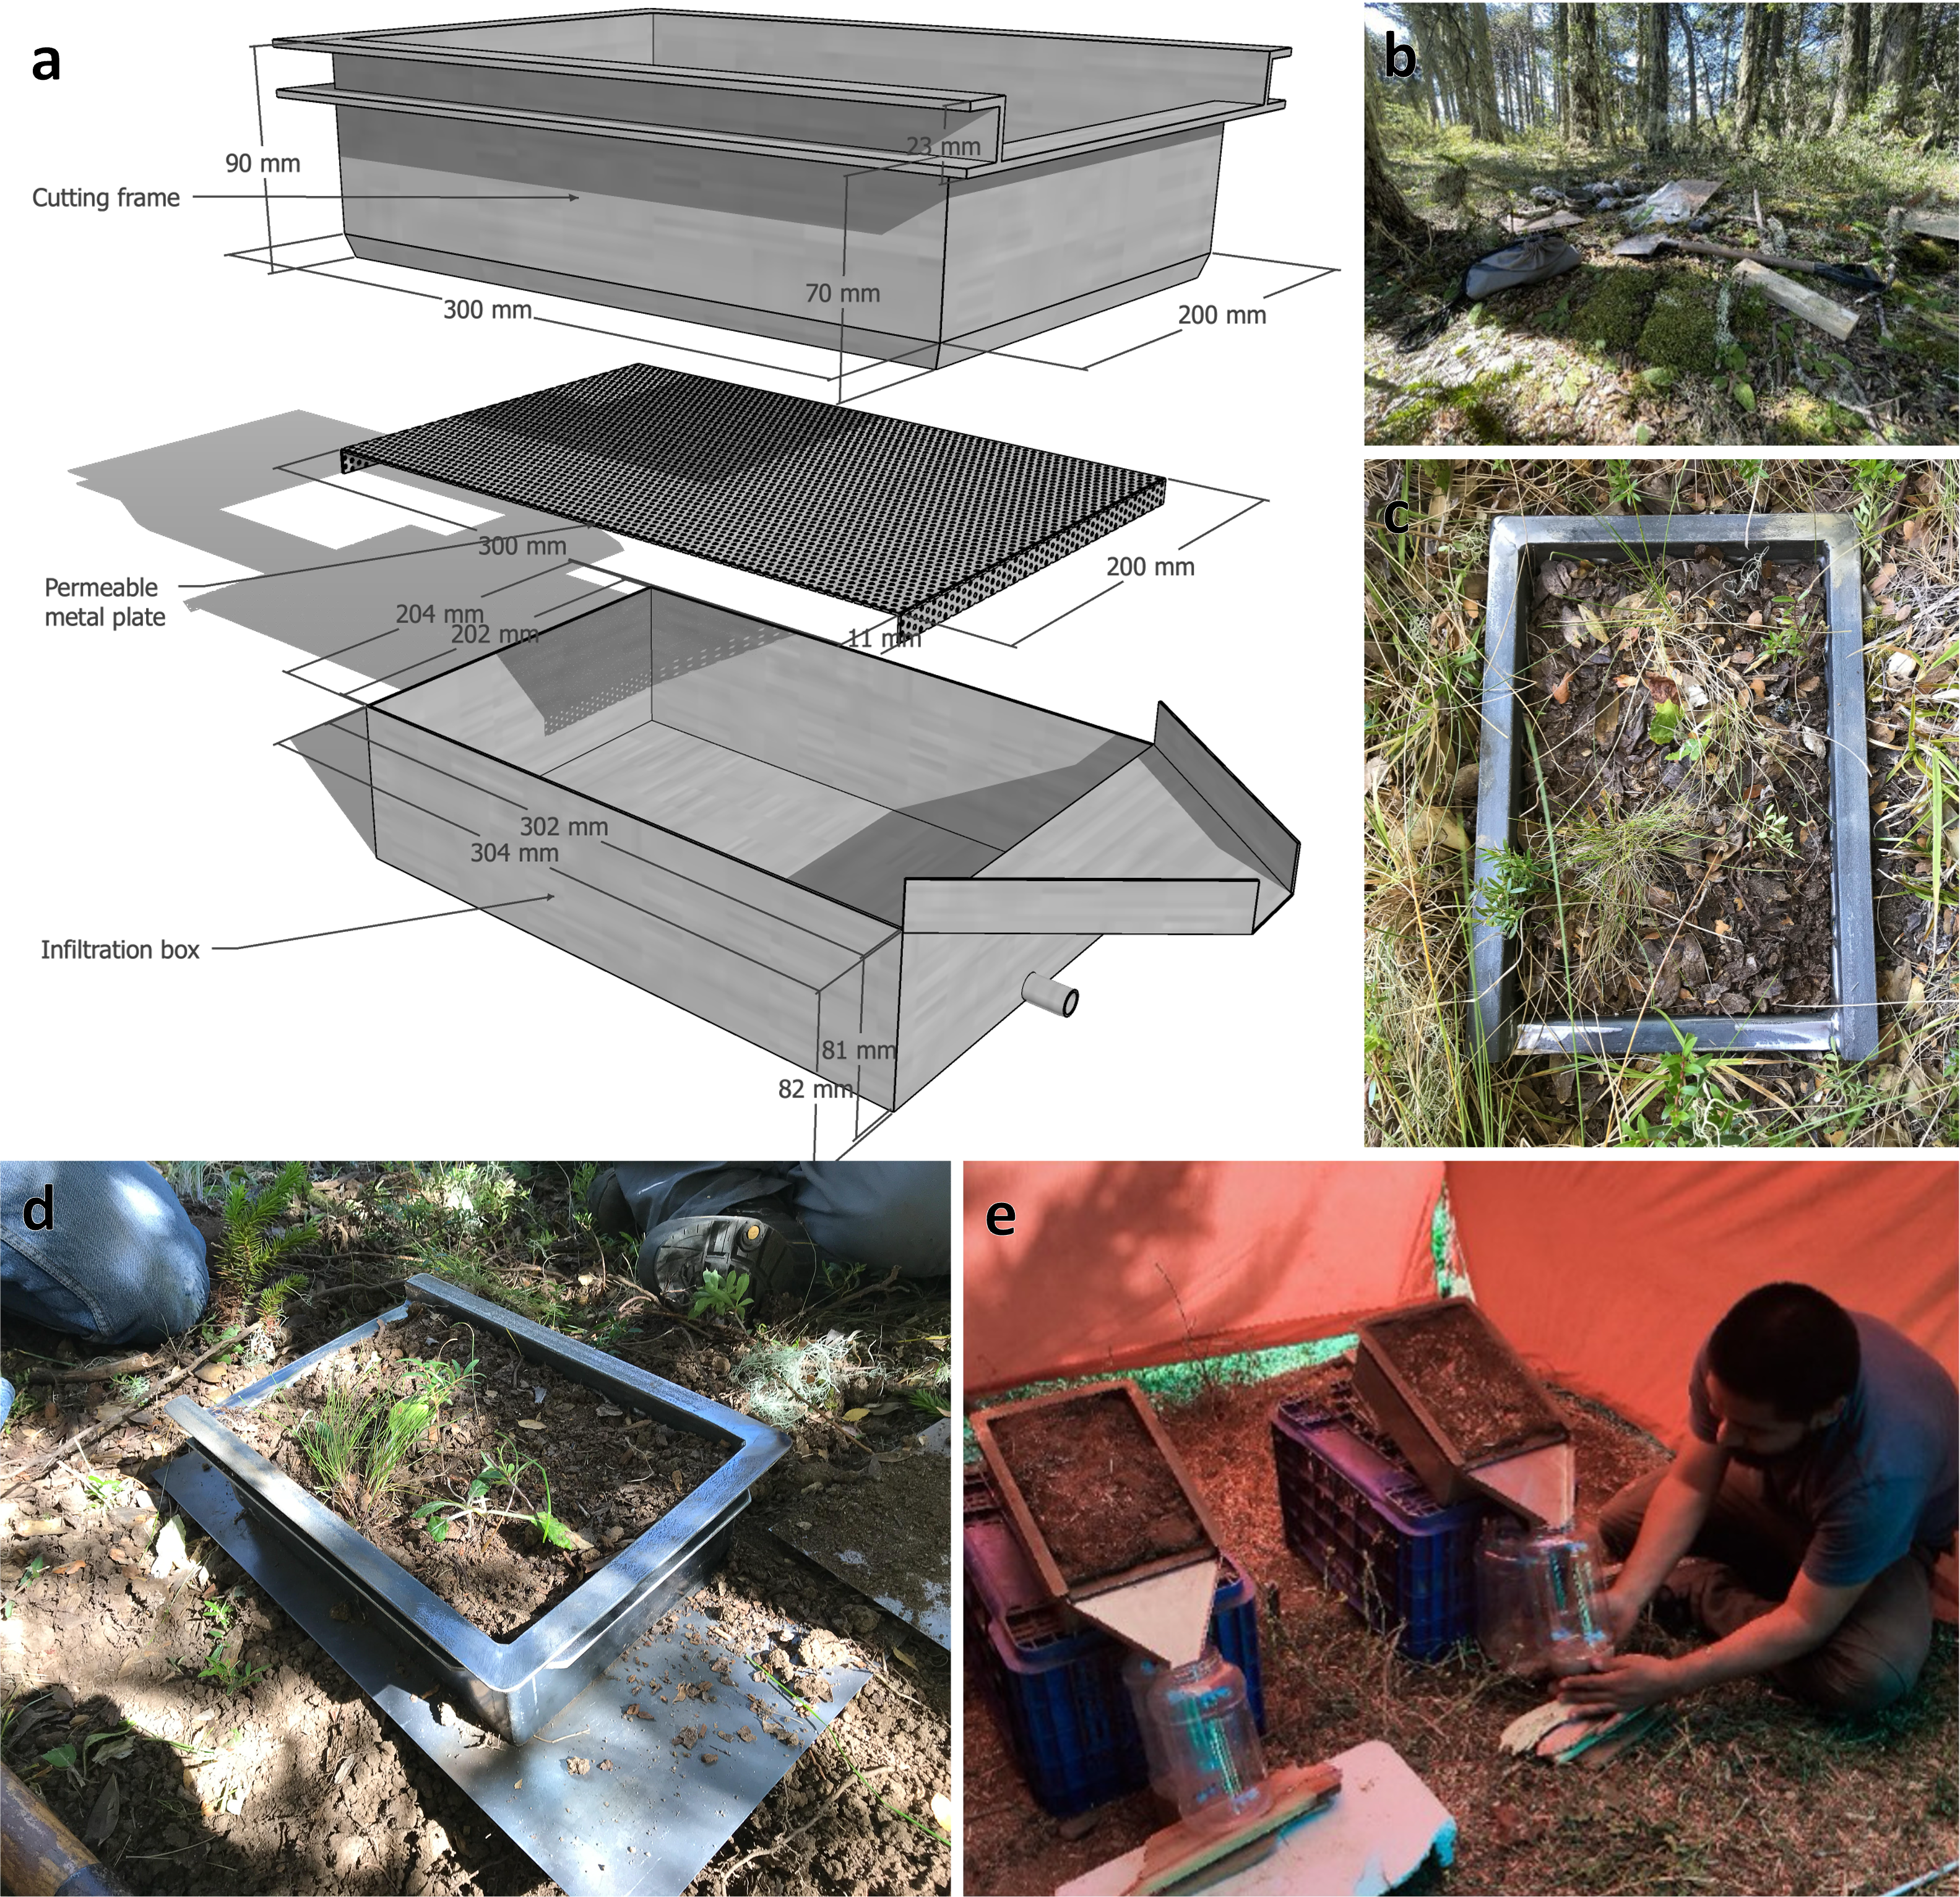
\includegraphics[width=1\textwidth]{img/sampling-panel.png}
	\caption[Field experimental setup for soil erosion and rainfall simulation: construction of the flux box, plot preparation, and biocrust evaluation at Nahuelbuta (NA)]{Construction diagram of the soil erosion flux box used in the experiment (a), general view of a plot with the presence of biocrust prior to sampling (b). (c, d) shows an installed cutting frame and the cleared and prepared soil. (e) demonstrates the setting for rainfall simulations at the Nahuelbuta (NA) study site.}
	\label{fig:sampling-panel}
\end{figure}

\FloatBarrier

Rainfall simulations were conducted near the sampling locations using the T\"ubingen rainfall simulator \citep{Iserloh2013,Seitz2015} equipped with a Lechler 460.788.30 nozzle and set to a falling height of \SI{3.5}{\meter}. Infiltration boxes were placed inside the simulator on a \ang{10} slope (Figure \ref{fig:sampling-panel}e). A rainfall event was simulated using an intensity of \SI{45}{\milli\metre\,\hour^{-1}} sustained over a 30‐minute period. According to regional intensity-duration-frequency analyses for central Chile \citep{PizarroTapia2020}, such an intensity falls within the extreme rainfall category, well above the heavy precipitation threshold even for relatively wet climates. This extreme intensity was selected to exceed the soil infiltration capacities and reliably generate surface runoff at all study sites. The time to initial runoff and percolation was recorded. Runoff and sediment-laden water samples were collected separately. Runoff volume was measured using a graduated beaker. Samples were allowed to settle by gravity for 12 hours, after which a water sample was extracted from the supernatant via siphoning, frozen at \SI{-4}{\celsius} and transported to the University of T\"ubingen for DOC and DON analysis. The remaining sediment was oven-dried at \SI{105}{\celsius} for 48 hours after all visible moisture was removed, then weighed. Sediment load was determined by dividing the dry sediment weight by the corresponding runoff volume and transported to the University of T\"ubingen for total C and N analyses. 

\section{Laboratory methods}
\subsection{Baseline soil characterization}

Before commencing experimental manipulations, a suite of baseline soil properties was determined on the sieved ($<$\SI{2}{\milli\metre}), air-dried field samples. Physical properties measured included bulk density (BD), determined gravimetrically, and particle size distribution (PSD). PSD was analyzed following the method of \citet{Kohn1929}, which combines sieving for fractions larger than \SI{20}{\micro\metre} with pipetting for fractions smaller than \SI{20}{\micro\metre} (Manuscript 1). Soil texture classes were subsequently interpreted based on World Reference Base (WRB) guidelines \citep{Jahn2006}. Chemical properties assessed included soil pH and electrical conductivity (EC), measured in soil:water suspensions (1:2.5 or 1:5 ratios) using calibrated meters (Manuscripts 1, 3 and 5). Total carbon (C\textsubscript{T}) and total nitrogen (N\textsubscript{T}) contents were quantified via oxidative heat combustion at high temperatures (\SI{1150}{\degreeCelsius}) using an elemental analyzer (Vario EL III, Euro EA) (Manuscripts 1, 3, 4 and 5). Soil organic carbon (SOC) was typically calculated by subtracting the inorganic carbon (SIC) content from the C\textsubscript{T} content. SIC was measured using a calcimeter (Scheibler method) or determined through acid digestion, particularly for soils with pH values exceeding 6.7--7.0 (Manuscripts 1, 3 and 4). Additionally, concentrations of various inorganic ions (Cl$^{-}$, NO$_{3}^{-}$, PO$_{4}^{3-}$, SO$_{4}^{2-}$, Na$^{+}$, Ca$^{2+}$) were measured in soil leachates prepared from the samples, utilizing ion chromatography (IC) (Manuscript 3).

\subsection{Aggregate stability}

Various methods were utilized to evaluate soil aggregate stability and to physically separate soil into different fractions based on aggregate size or density, tailored to the specific research objectives of each study. To assess overall aggregate stability across the climate gradient (Manuscript 1), a large-sample (\SI{200}{\gram}, homogenized $<$\SI{30}{\milli\meter}) two-stage sieving method based on \citet{Hartge2009} and \citet{Six2000} was employed. Samples underwent initial dry sieving through a nested stack of sieves (ranging from \SI{19.0}{\milli\meter} down to \SI{2.0}{\milli\meter}), followed by a repetition of the sieving process underwater. Water-stable aggregates (WSA\textsubscript{\SI{2.0}{\milli\meter}}) were determined, and several stability indices were calculated from the dry and wet sieving results. The difference in mean weight diameter (MWD), representing the average size of aggregates weighted by their mass proportion, was calculated as:

\begin{itemize}
  \item Difference in mean weight diameter ($\Delta$MWD)
    $$\Delta MWD = \frac{\sum_{i=1}^{n} X_i*W_i}{\sum_{i=1}^{n} W_i}$$
    were:
    \begin{itemize}
        \item $X_i$: The mean diameter of the stable aggregate fraction $i$.
        \item $W_i$: The corrected mass proportion of the stable aggregate fraction $i$ within the total considered range (e.g., 2-30 mm).
        \item $n$: The total number of aggregate size fractions being analyzed.
    \end{itemize}
  \item Difference in geometric mean diameter ($\Delta$GMD):
    $$\Delta GMD = exp \left[\frac{\sum_{i=1}^{n} X_i\lg W_i}{\sum_{i=1}^{n} W_i}\right]$$
    were:
    \begin{itemize}
        \item $X_i$: The mean diameter of the stable aggregate fraction $i$.
        \item $W_i$: The corrected mass proportion of the stable aggregate fraction $i$ within the total considered range (e.g., 2-30 mm).
        \item $n$: The total number of aggregate size fractions being analyzed.
    \end{itemize}
  \item Water stability aggregate ratio (WSAR):
    $$WSAR = \frac{WSA}{A}*100$$
    were:
    \begin{itemize}
        \item $WSA$: The content (mass or weight) of water-stable aggregates larger than 2 mm after a stability test.
        \item $A$: The content (mass or weight) of dry aggregates larger than 2 mm before the stability test.
    \end{itemize}
  \item Proportion of soil macroaggregate of a diameter less than 2 mm (R$_{<2mm}$)
    $$R_{<2mm}=\frac{W_{r>2}}{W_T}*100 = \left(1-\frac{W_{r<2}}{W_T}\right)$$
    were:
    \begin{itemize}
        \item $W_{r>2}$: The content (mass or weight) of water-stable aggregates larger than 2 mm after a stability test.
        \item $W_T$: The content (mass or weight) of dry aggregates larger than 2 mm before the stability test.
        \item $W_{r<2}$: The weight of microaggregates and primary particles with a diameter less than 2 mm.
    \end{itemize}
\end{itemize}

For other investigations focusing on aggregate turnover dynamics and the association of microbial communities or organic matter with specific aggregate sizes (Manuscripts 3, 4 and 5), wet sieving techniques were applied to smaller soil samples (\SIrange{5}{10}{\gram}). One approach utilized a modified Casagrande apparatus, shaking \SI{5}{\gram} of soil on stacked sieves (\SIrange{250}{53}{\micro\metre}) through 1000 cycles at \SI{2}{\hertz}. This yielded fractions defined as macroaggregates ($>$\SI{250}{\micro\metre}), large microaggregates (\SIrange[range-phrase=--,range-units=single]{250}{53}{\micro\metre}), and a combined fraction of small microaggregates and primary particles ($<$\SI{53}{\micro\metre}) (Manuscript 3). Another frequently used method, adapted from \citet{Elliott1986}, involved pre-wetting \SI{10}{\gram} of soil, followed by manual immersion sieving. This typically involved moving a stack of sieves ($>$\SI{500}{\micro\metre}, \SIrange[range-phrase=--]{500}{250}{\micro\metre}, \SIrange[range-phrase=--,range-units=single]{250}{53}{\micro\metre}, \SIrange[range-phrase=--,range-units=single]{53}{20}{\micro\metre}) gently up and down in water for a set number of repetitions (30 strokes over 5 minutes), with the finest fraction ($<$\SI{20}{\micro\metre}) captured on a filter paper (Manuscript 4). Following separation by either method, the recovered aggregate fractions were carefully oven-dried (at \SI{40}{\degreeCelsius} or \SI{105}{\degreeCelsius}) and weighed. The MWD was often calculated from the resulting mass distribution across the obtained size classes.

To isolate soil organic matter (SOM) pools based on their physical protection and association with minerals (Manuscript 5), density fractionation was performed. This procedure typically used sodium polytungstate (SPT) solution at an adjusted density of \SI{1.8}{\gram\,\centi\metre^{-3}}. Bulk soil or pre-defined aggregate fractions were suspended in the SPT solution, allowing the lighter, free particulate OM (fPOM) to float and be separated. Subsequently, ultrasonic dispersion (using an energy input of \SI{440}{\joule\,\milli\litre^{-1}}) was applied to break apart remaining aggregates and release occluded POM (oPOM). This oPOM was then further separated by wet sieving into 3 different size classes ($>$\SI{63}{\micro\metre}, 63-\SI{20}{\micro\metre}, $<$\SI{20}{\micro\metre}). The dense mineral material remaining after these separation steps constituted the mineral-associated OM (MAOM). All physically separated SOM fractions were thoroughly rinsed to remove the SPT, dried, and weighed. The SOC, C\textsubscript{T} and N\textsubscript{T} contents of these individual aggregate size or density fractions were then determined using elemental analysis, providing crucial information on carbon and nitrogen storage and distribution within the soil's physical structure (Manuscripts 3, 4 and 5). In addition, stable isotope analysis ($\delta^{13}\mathrm{C}$, $\delta^{15}\mathrm{N}$) was conducted on density fractions to elucidate the sources and transformation pathways of the organic matter (Manuscript 5).

\subsection{Incubation experiments}

Controlled laboratory incubations were central to simulating specific environmental scenarios or distinct stages of soil succession. To mimic a climate change scenario involving a shift to more humid conditions for arid and semi-arid soils (Manuscript 3), soil microcosms were established using sterilized PVC columns filled with \SI{130}{\gram} of sieved soil. These were incubated under controlled diurnal temperature fluctuations, a 14/\SI{10}{\hour} day/night photoperiod, and a defined moisture regime involving rewetting to 65\% water-filled pore space (WFPS) three times per week, reflecting conditions of the humid Nahuelbuta (NA) site. Experimental treatments encompassed sterile controls, native soil containing indigenous microorganisms (\textit{in situ}), native soil where biocrusts were allowed to develop (BSC), and native soil cultivated with a pioneer plant species (\textit{Helenium aromaticum}). Destructive sampling of microcosms occurred at baseline (T0) and after 2, 12, and 16 weeks of incubation. To specifically assess the impact of differing moisture regimes on soil properties and microbial communities (Manuscript 4), native and sterilized soils (\SI{60}{\gram}) were incubated in Tübingen cups (T-cups) for a total of six weeks. Treatments included repeated wetting-drying (WD) cycles and a constant moisture (CM) condition. WD cycles involved saturating the soil to field capacity (pF 1.8), allowing it to air-dry (\SI{25}{\degreeCelsius}, 1-2 days), and then re-saturating it by placing the T-cup on a sterile sand bed. CM samples remained continuously saturated on the sand bed. Sampling points included the initial state (R0) and after one, three, and six WD cycles (R1, R3, R6), as well as after six weeks under constant moisture (CM). For studying the transition from a living root system to a decomposing one (Manuscript 5), an experiment focusing on rhizosphere and detritusphere dynamics was conducted. Semi-arid topsoil and subsoil were incubated in pots, either with or without the pioneer plant \textit{Helenium aromaticum}, under greenhouse conditions for 70 days (representing the rhizosphere phase). Following this, the aboveground plant biomass was clipped at the soil surface, and the pots were moved to darkness at room temperature for an additional 100 days, allowing the roots and shoots to decompose in situ (representing the detritusphere phase). Soil samples were collected at the conclusion of both the rhizosphere and detritusphere phases, carefully separating root-adhering soil from bulk rhizosphere/detritusphere soil where feasible.

\subsection{Molecular analyses}

The abundance and composition of microbial communities were investigated using quantitative PCR (qPCR) and high-throughput amplicon sequencing. Total genomic DNA was extracted from soil samples (typically \SIrange[range-phrase=--,range-units=single]{0.25}{0.5}{\gram} per extraction), often in duplicate or triplicate, using commercially available kits like the DNeasy PowerSoil Kit (Qiagen), adhering to the manufacturer's protocols (Manuscripts 3 and 4). The abundance of major microbial groups – bacteria, archaea, and fungi – was quantified by qPCR targeting specific ribosomal RNA gene fragments. Commonly used primer pairs included Eub341F/Eub534R for bacterial 16S rRNA genes, 340F/1000R for archaeal 16S rRNA genes, and NL1F/LS2R for fungal 28S rRNA genes or ITS region primers. qPCR assays were performed using SYBR Green-based detection on real-time PCR platforms (Bio-Rad CFX96). Quantification relied on standard curves generated from serial dilutions of plasmids containing known copy numbers of the target gene. Rigorous quality control included monitoring reaction efficiencies and analyzing melt curves to ensure amplification specificity (Manuscripts 3 and 4). For detailed community composition analysis, the V4 hypervariable region of the 16S rRNA gene was typically amplified using universal primers (515F/806R) tagged with unique barcodes for sample multiplexing. Sequencing was performed using the Illumina MiSeq platform, generating paired-end reads (2x300bp) (Manuscripts 3 and 4). The resulting raw sequence data underwent a standardized bioinformatics pipeline. This involved demultiplexing reads based on barcodes (eusing cutadapt), performing quality filtering and trimming, merging paired-end reads (where applicable), identifying and removing chimeric sequences, and generating Amplicon Sequence Variants (ASVs) using algorithms like DADA2. Taxonomic classification of ASVs was achieved by comparison against established reference databases, primarily SILVA. Sequences identified as originating from chloroplasts, mitochondria, or represented by only a single read (singletons) were typically removed from the final dataset (Manuscripts 3 and 4). In some cases, potential ecological functions of the identified prokaryotic taxa were inferred using predictive tools such as FAPROTAX (Manuscript 4).

\subsection{Organic matter and microbial biomarker characterization}

To gain deeper insights into the composition of soil organic matter (SOM) and the structure of microbial communities, advanced analytical techniques were employed. The chemical composition of bulk plant material and specific SOM pools isolated via density fractionation (POM fractions) was characterized using solid-state $^{13}$C Cross-Polarization Magic Angle Spinning (CP-MAS) Nuclear Magnetic Resonance (NMR) spectroscopy. The resulting spectra were quantified based on established chemical shift regions corresponding to major biochemical classes, including alkyl C, O-alkyl C, aromatic C, and carbonyl C. Diagnostic indices, such as the alkyl C/O-alkyl C ratio, were calculated to infer OM composition and degradation state. Additionally, a Molecular Mixing Model (MMM) was sometimes applied to estimate the relative contributions of broader biochemical categories like carbohydrates, proteins, lipids, and lignin to the overall OM (Manuscript 5).

The composition of lignin within plant and root biomass was specifically investigated through cupric oxide (CuO) oxidation. This method breaks down the lignin polymer into characteristic phenolic monomers (vanillyl (V), syringyl (S), and cinnamyl (C) units), which were then quantified using Gas Chromatography-Mass Spectrometry (GC-MS). Total lignin content was estimated based on the sum of these units (VSC), and diagnostic ratios, such as S/V, C/V, and acid-to-aldehyde ratios within each phenol group (e.g., (Ac/Al)$_\mathrm{V}$), were calculated to assess lignin source and degradation stage (Manuscript 5).

Phospholipid Fatty Acid (PLFA) analysis was used to characterize the structure and biomass of the active microbial community. Lipids were extracted from soil using methods like a modified Bligh \& Dyer extraction, and PLFAs were separated from neutral and glycolipids, often via solid-phase extraction. The purified PLFAs were then converted into Fatty Acid Methyl Esters (FAMEs) through transesterification and subsequently analyzed using Gas Chromatography coupled with Flame Ionization Detection (GC-FID). Specific FAMEs served as biomarkers for different microbial groups: e.g., 18:2$\omega$6,9 for fungi; iso- and anteiso-branched fatty acids for gram-positive bacteria; and monounsaturated or cyclic fatty acids for gram-negative bacteria. These data allowed for the calculation of total microbial biomass and structural indices such as the fungi:bacteria ratio and the gram$^{+}$:gram$^{-}$ ratio (Manuscript 5).

\section{Statistical analyses}

The statistical analyses across manuscripts 1 to 5 employed a range of methods to investigate the relationships between biocrusts, microbial communities, plant roots, and soil properties. Generalized linear models (GLMs) were commonly used to assess the influence of factors like climate, biocrust presence, and treatments on soil properties and aggregate stability (Manuscripts 1, 2 and 3). Model selection was based on the Akaike Information Criterion (AIC) and data characteristics, utilizing appropriate link functions (Gaussian, Gamma, inverse Gaussian, Tweedie) to account for non-normal distributions \citep{Dunn2017,RCoreTeam2018,Wickam2016}. Tukey’s post-hoc test was used for pairwise comparisons ($p < 0.05$).

Analysis of variance (ANOVA) and analysis of covariance (ANCOVA) were also employed, particularly to assess differences in measured properties between treatments and across sites or horizons. Where applicable, soil baseline variables were used as covariates in ANCOVA (Manuscripts 2 and 5). Non-parametric tests, such as the Kruskal-Wallis test followed by Mann-Whitney post-hoc tests, were used when normality or homoscedasticity assumptions were violated (Manuscript 3). Data transformations were applied when necessary, using the $bestNormalize$ package \citep{Peterson2021,Peterson2020}. The Dunn-Šidák correction was implemented for multiple comparisons \citep{Hothorn2008}.

Microbial community data were analyzed using various multivariate techniques. Non-metric multidimensional scaling (NMDS) was used to visualize community structure and beta diversity \citep{Oksanen2013}. Permutational multivariate analysis of variance (PERMANOVA) assessed the significance of differences between groups (e.g., sites, horizons, time points), often followed by pairwise PERMANOVA for detailed comparisons \citep{MartinezArbizu2020} (Manuscripts 3 and 4). Distance-based redundancy analysis (dbRDA) identified environmental factors influencing community composition (Manuscript 4). Indicator species analysis revealed taxa associated with specific sites or horizons using the $indval$ function \citep{Dufrene1997,Roberts2016} (Manuscript 4).

Co-occurrence networks explored the complex relationships within microbial communities. Network properties, including modularity, connectance, and hub species, were calculated using the $igraph$ package \citep{Csardi2006}, and correlations between ASVs were assessed using Pearson correlation \citep{Harrell2019} (Manuscript 4). Weighted gene co-expression network analysis (WGCNA) grouped highly correlated ASVs into modules to explore their relationships with physicochemical properties \citep{Langfelder2008} (Manuscript 4).

Molecular mixing models were used to quantify the relative contributions of different organic matter components (carbohydrates, proteins, lignin, lipids) based on 13C NMR spectroscopy data \citep{Nelson2005,Prater2020} (Manuscript 5).
